\chapter{Time-series analysis: background and theory}
\chaptermark{Time-series analysis}
\label{ch:litreview}
\label{ch:theory}

\begin{instructions}
Merged 5 Nov from the time-series half of the old Chapter 2 and all of the old Chapter 3 (theory), in the agreed
order: nomenclature; frequency, wavelets and (one paragraph of) entropy; matrix profiling, trimmed; image encodings and
CNNs; classifiers without hand-crafted features (MiniRocket); detectors borrowed from other fields; distance and scale;
surrogates; human judgement; evaluation statistics; gaps. The excitable-system models section is cut with the
modelling. About 10--12 pages. Every new method cited in Chapters~\ref{ch:rq1}--\ref{ch:roundb} needs its source here.
Bibliography entries added on 2026-10-26 are marked VERIFY in \src{docs/thesis/bib/thesis.bib}; check each against the
paper.
\end{instructions}

This chapter reviews the time-series methods used in this thesis and sets out the theory they rest on. Section~\ref{sec:nomenclature} introduces the vocabulary of time-series analysis. Sections~\ref{sec:frequency} to~\ref{sec:litclassifiers} cover the techniques that produce features, matches and classifications, and Section~\ref{sec:litdetectors} reviews the detectors borrowed from other fields. Sections~\ref{sec:distance} to~\ref{sec:stats} cover the distances, nulls, human judgements and statistics that turn their outputs into findings, and Section~\ref{sec:litgaps} consolidates the gaps.

\begin{instructions}
Bridging paragraph drafted 5 Nov from the two old chapter openings; rewrite it in your words in the writing loop.
\end{instructions}

\section{Time-series analysis and its nomenclature}
\label{sec:littsa}
\label{sec:nomenclature}

In today's information age, time-series analysis is a quickly growing field with many exciting concepts for extracting information from ever-more complex dynamical systems \cite{cabauatan}, \cite{gao}. Traditional methods of decomposition and smoothing --- including autoregressive integrated moving average (ARIMA) models and autocorrelation-based approaches --- assume that the statistical properties of a signal do not change over time, a property which is often violated by biological signals such as those produced by mycelium networks. The field has consequently moved towards more flexible methods involving machine learning and feedback-based approaches, leveraging the increase in processing power and memory available today \cite{gao}, \cite{milvus}.

A time series $T$ is defined as a sequence of real-valued numbers $x_i : T = x_1, x_2, \ldots, x_n$ recorded at evenly spaced time intervals $(t_1, t_2, \ldots, t_n)$ where $n$ is the length of $T$. Time series data, for analysis purposes, is equally sampled in time. A motif, or shapelet, is a subsequence of the time series $T$ that is of particular interest.

Broadly speaking, time-series analysis techniques fall into several main categories, based on their primary objective and the type of information they are designed to extract.

\textbf{Classification} techniques involve assigning subsequences to defined categories based on their respective characteristics. This is a common technique for data that is already labelled, allowing a model to train on a labelled dataset and learn the common features within each category. Classification for bio-electric signals may be used to help identify different types of spiking behaviour or responses to stimuli.

\textbf{Clustering} is an unsupervised learning approach that groups similar time-series or subsequences together without predefined labels. The goal is to discover natural categories within the data based on similar characteristics. This can be useful for identifying recurring patterns or families of signal behaviour in fungal electrical activity.

\textbf{Segmentation} involves dividing a time-series into meaningful regions or segments, where each segment exhibits relatively consistent behaviour. This is particularly useful for detecting changes in signal dynamics, such as transitions between inactive periods and active spiking regions.

\textbf{Motif discovery} focuses on identifying frequently occurring subsequences within a time-series. These motifs, also known as shapelets, can represent characteristic patterns of interest. In biological signals, motifs may correspond to repeated signalling structures or functional events.

\textbf{Anomaly detection} aims to identify unusual or rare patterns that deviate significantly from normal behaviour. These anomalies may represent noise, experimental artefacts, or meaningful but infrequent biological events.

\textbf{Forecasting} involves predicting future values of a time-series based on its past behaviour. This can range from simple statistical models to complex machine learning approaches. In the context of this project, forecasting may provide insight into the predictability of fungal electrical activity.

\begin{instructions}
Add one sentence on uneven sampling. Several recordings in the corpus have uneven time axes: MJu26a's gaps range from
0.124 to 2.83\,s. They are interpolated onto a uniform grid at their native rate (Section~\ref{sec:preprocessing}),
not reduced to 1\,Hz as the plan assumed.
\end{instructions}

\section{Frequency, wavelet and entropy analysis}
\label{sec:frequency}

Many signals in the time domain exhibit structure and information in the frequency domain. Through analysis techniques such as the Fourier transform, and Wavelet transforms, information about the frequencies present, at what time and at what strength can be uncovered, exposing the oscillatory foundations of a dataset.

A Fourier Transform represents a time-series signal as a weighted sum of sinusoidal components at different frequencies, mapping the signal into the frequency domain via the transformation:
\begin{equation}
X(j\omega) = \int_{-\infty}^{\infty} x(t) e^{-j\omega t}\,dt
\end{equation}

For discrete datasets such as time-series data, the Discrete Fourier Transform is used via the Fast Fourier Transform algorithm, an efficient algorithm for computing the Discrete Fourier Transform that reduces computational complexity from $O(n^2)$ to $O(n \log n)$.

A drawback of the FFT is that it assumes the statistical properties of a signal do not change over time, a property which is often violated by biological signals which are non-stationary. Such signals are analysed via the Short-Time Fourier Transform, which applies a small overlapping sliding window to the signal to apply the FFT algorithm, formally defined as:
\begin{equation}
X(t,\omega) = \int x(\tau) w(\tau - t) e^{-i\omega\tau}\,d\tau
\end{equation}

With the STFT, the frequency content can be tracked over time, often visualised via a spectrogram. A STFT has a large trade-off between frequency resolution and time resolution, meaning that it is often still difficult to analyse events at individual points in time across multiple scales.

A Wavelet transform is a more flexible approach for decomposing a signal into its frequency components by instead using localised functions called wavelets. The Continuous Wavelet Transform (CWT) represents a signal as:
\begin{equation}
W(a,b) = \int x(t)\,\psi^{*}\!\left(\frac{t-b}{a}\right)dt
\end{equation}
where $a$ is the scale parameter, $b$ is the translation parameter, and $\psi$ is the mother wavelet.

Wavelet transforms are well-suited for signals with spikes and bursts, as higher-frequency components are analysed with fine temporal resolution, and lower-frequency components are analysed over longer durations. This makes Wavelet analysis particularly suitable for the behaviours exhibited in the biological signals of mycelium. It is the basis of the band decomposition and wavelet detectors in the sweep (Chapter~\ref{ch:rq1}), and of the Dehshibi detector \cite{dehshibi}.

\paragraph{Entropy and complexity.}
\label{sec:entropy}
Entropy-based methods attempt to quantify the complexity and unpredictability of time-series data. The results generated by entropy analysis indicate whether a signal exhibits random or patterned structure in the values over time. Shannon entropy is the fundamental measure, the average uncertainty of the signal's values. Other types of entropy include Permutation Entropy, SVD Entropy and Spectral Entropy, and Sample and Approximate Entropy evaluate whether similar patterns in a dataset remain similar over time, providing another measure of regularity.

\begin{instructions}
Cut to one paragraph on 5 Nov: multiscale entropy (B7) is not reported. Entropy features appear only in the early
window matrix and in the random forests' 24-feature set (catch22 plus fast entropy, Chapter~\ref{ch:early}). Name the
ones used, from the feature code in \src{Working/training/}, in one sentence.
\end{instructions}

\section{Matrix profiling}
\label{sec:litmp}
\label{sec:mp}

Time series motif discovery is a complex problem whose results influence classification, clustering and rule discovery \cite{linardi}. The Matrix Profile algorithm was first proposed in 2016 by the University of California, Riverside by a collection of authors including Chin-Chia Michael Yeh and Eamonn Keogh \cite{yeh}. Building on existing work in the field of all-pairs similarity searching, they propose an efficient parallelisable method for large time-series datasets that reduces the previously prohibitive $O(n^2)$ complexity to $O(n\log n)$ via the STOMP and SCRIMP++ algorithms \cite{stumpy}. The core output of the matrix profile is a vector storing the nearest neighbour distance for every subsequence in the dataset: low values indicate locations of recurring motifs, and high values indicate discords --- anomalous or rare subsequences. A key advantage of this technique is that it is exact, guaranteeing the most similar patterns are discovered, unlike earlier approximation-based approaches.

To compute a Matrix Profile from a given time-series sequence of length $n$, all sub-sequences of a fixed length beginning at every index $i \in [1,n]$ are compared to each other. At each index, the lowest computed distance to another subsequence in the set is recorded. This produces a plot that highlights where very similar structural motifs are evident, and also where very rare motifs or anomalies may be (termed as \emph{discords}).

Crucially, before the introduction of the Matrix Profile, there were no attempts to discover motifs more than approximately 900 data points long \cite{zhu2020}. At a sampling rate of 1\,Hz, mycelium motifs of interest span 60 to 3600 data points (1 minute to 1 hour), placing them squarely in the range that matrix profiling first made tractable. This makes the technique particularly well-suited to the analysis of bio-electric signals in fungi.

A number of extensions to the core algorithm are of relevance to this project. Time Series Chains \cite{zhu2017} detect evolving or drifting motifs, which is relevant to the slow biological trends in mycelium signals where waveform shape may shift gradually over many hours. Variable-length motif discovery \cite{linardi} removes the requirement for a fixed subsequence length, which is important given that spike duration in mycelium varies across both time and species. The pan matrix profile \cite{madrid2019pan} computes the profile at every length in a range, and FLUSS \cite{gharghabi2017fluss} uses the profile's arc structure for semantic segmentation without labels. MPdist \cite{gharghabi2018mpdist} turns the profile into a distance between whole series that tolerates differences in length.

The fact that matrix profiling can support such a wide range of information-producing computations makes it a powerful tool for analysing an unpredictable, non-stationary signal like those produced by mycelium networks. Its use cases have extended across many domains, and several of these are directly analogous to the problem at hand. Shi et al.\ \cite{shi} applied it to power systems synchrophasor data to automatically discover and label event types without prior templates --- a setting that is structurally very similar to the present problem, where signal events are non-stationary and not catalogued in advance. Ponganis et al.\ \cite{ponganis} used matrix profiling for respiratory cycle identification in penguins without requiring manually defined breath templates. Liu et al.\ \cite{liu} applied discord detection to Apollo seismic data to identify rare anomalous events in long recordings. Athira et al.\ \cite{athira} applied matrix profiling to multi-channel recordings of \emph{Ciona intestinalis} behavioural dynamics, a setting that is most structurally similar to the multi-electrode mycelium data used in this project.

A key advantage for the present project is that matrix profiling requires no labels, meaning motifs can be discovered in a fully unsupervised manner. It is also the mechanism underlying seeded search (RQ2): an exemplar accepted by a human can be used directly as a query, and the resulting matches presented for adjudication.

A seeded search uses a single query $Q$, an exemplar chosen by a human, instead of all subsequences. It computes the distance profile $D_Q(i) = d_z(Q, T_{i,m})$ against every subsequence $T_{i,m}$ of length $m$, and keeps every position below a threshold as a match. The cost is that of one row of the matrix profile, $O(n \log n)$ with the MASS algorithm. That is why a query against 721 hours of 16 channels takes seconds, where the full profile takes days.

\begin{instructions}
Add one sentence on cost, from this project. A whole-signal matrix profile on this machine is estimated at about 40\,h
for M2\_concat and 260\,h for M2\_aug. A seeded search takes about 4\,s per query. This is why seeded search became the
practical cross-channel method (memory note: m2-datasets-and-seeds).
\end{instructions}

\begin{instructions}
Trimmed 5 Nov: the old theory chapter's restatements of the 2016 origin and the ``guarantees the most similar
patterns'' advantage were dropped, as the paragraphs above already say both.
\end{instructions}

\begin{figure}[htbp]
\centering
\figplaceholder{5cm}{Figure 2.1 (T2, bundle + \src{Results/Detection/matrix_profile/_legacy/}): one day of M2\_concat CH0
with its 10-minute matrix profile underneath (no new computation), the top motif pair boxed on the trace and overlaid
z-normalised beside it.}
\caption{What a matrix profile shows: low values mark subsequences with a close match elsewhere.}
\label{fig:mpintuition}
\end{figure}

\section{Image encodings and convolutional networks}
\label{sec:litnn}
\label{sec:encodings}

Neural networks are a popular choice for time-series classification tasks due to their accuracy and flexibility \cite{bagnall}. Recurrent architectures such as LSTMs were initially favoured for sequential data, however Convolutional Neural Networks (CNNs) have become competitive --- and in many cases superior --- when time-series data is first encoded as a two-dimensional image. By converting a time-series into a structured image representation, the well-developed image classification capabilities of CNNs can be directly applied to temporal data. Some of the more common methods for transforming time-series data into images are Recurrence Plots, Gramian Angular Fields, Markov Transition Fields, and spectrograms generated via the Continuous Wavelet Transform or Short-Time Fourier Transform. Each captures a different structural property of the signal, and choosing among them for a given domain is non-trivial.

In the field of EEG analysis, studies on the implementation of Neural Network models in classification have been published since as early as 2016 \cite{mohammed}. A study in the University of Thi-Qar Journal for Engineering Sciences \cite{mohammed} surveyed the current collection of machine learning algorithms in EEG analysis, finding that some of the more powerful algorithms achieved accuracies of over 90\%, and discussed hybrid models achieving up to 99\% accuracy and sensitivity. A separate study performed by Murungi et al.\ \cite{murungi} highlighted that the field of machine learning within EEG analysis is largely a result of the abundance of high-quality readily available datasets, another factor which the field of mycelium signal analysis lacks. They found that the most popular algorithm for Neural Network analysis was Convolutional Neural Networks, often trained on EEG spectrograms, followed closely by Recurrent Neural Networks (RNNs).

In the paper by Mariani, Appiah and Tweneboah \cite{mariani}, they propose a new methodology for image creation for the purpose of training a CNN, combining a Gramian Angular Difference Field, Gramian Angular Summation Field and Recurrence plot into a single three-channel RGB input, and using Bayesian optimisation for hyperparameter tuning. They claim that fusion plots enrich the structural encoding of temporal dynamics, finding that on seven separate univariate datasets, their method significantly outperforms other classification algorithms such as Dynamic Time Warping (DTW) and Shapelet Transforms. The datasets used are also non-stationary, including facial outlines mapped into 1D series and word height profiles, but none have behavioural characteristics similar to bio-electric signals.

A neural network is a machine-learning model designed to approximate a function. For any input vector $X = (x_1, x_2, \ldots, x_n)$ find a function $f(X)$ that maps the vector to $Y$. This is achieved by layers of neurons that find correct weights --- a measure of an input's influence on the outcome --- and the correct biases --- values that shift the decision threshold \cite{ibmnn}.

Gramian Angular Field transformations are the process of converting a set of time-series data $T$ into a Gramian matrix in the following process \cite{rgbgaf} \cite{devitry}. The time series is first normalised to between $[-1,1]$, then converted into polar format:
\begin{align}
T &\leftarrow \mathrm{Normalise}(T)\\
r_i &= \frac{t_i}{t_n}, \qquad \theta_i = \arccos(x_i)
\end{align}

There are then two types of Gramian Matrices. The Gramian Angular Summation Field (GASF) computes every entry of the $(n,n)$ matrix as $(i,j) \leftarrow \cos(\theta_i + \theta_j)$, and the Gramian Angular Difference Field (GADF) computes every entry as $(i,j) \leftarrow \sin(\theta_i - \theta_j)$. The recurrence matrix is calculated as \cite{recurrence}:
\begin{equation}
(i,j) \leftarrow
\begin{cases}
1 & \text{if } |x_i - x_j| \leq \epsilon\\
0 & \text{else}
\end{cases}
\end{equation}
for some $\epsilon$.

Each of these encodings produces a square image from a window of signal, which can then be presented to a CNN as a single-channel input, or stacked as the three channels of an RGB image in the fusion approach of Mariani et al.\ \cite{mariani} (Figure~\ref{fig:encodings}). The models in this thesis resize each image to $224\times224$ and classify it with an ImageNet-pretrained EfficientNet-B0 \cite{tan2019efficientnet}.

\begin{figure}[htbp]
\centering
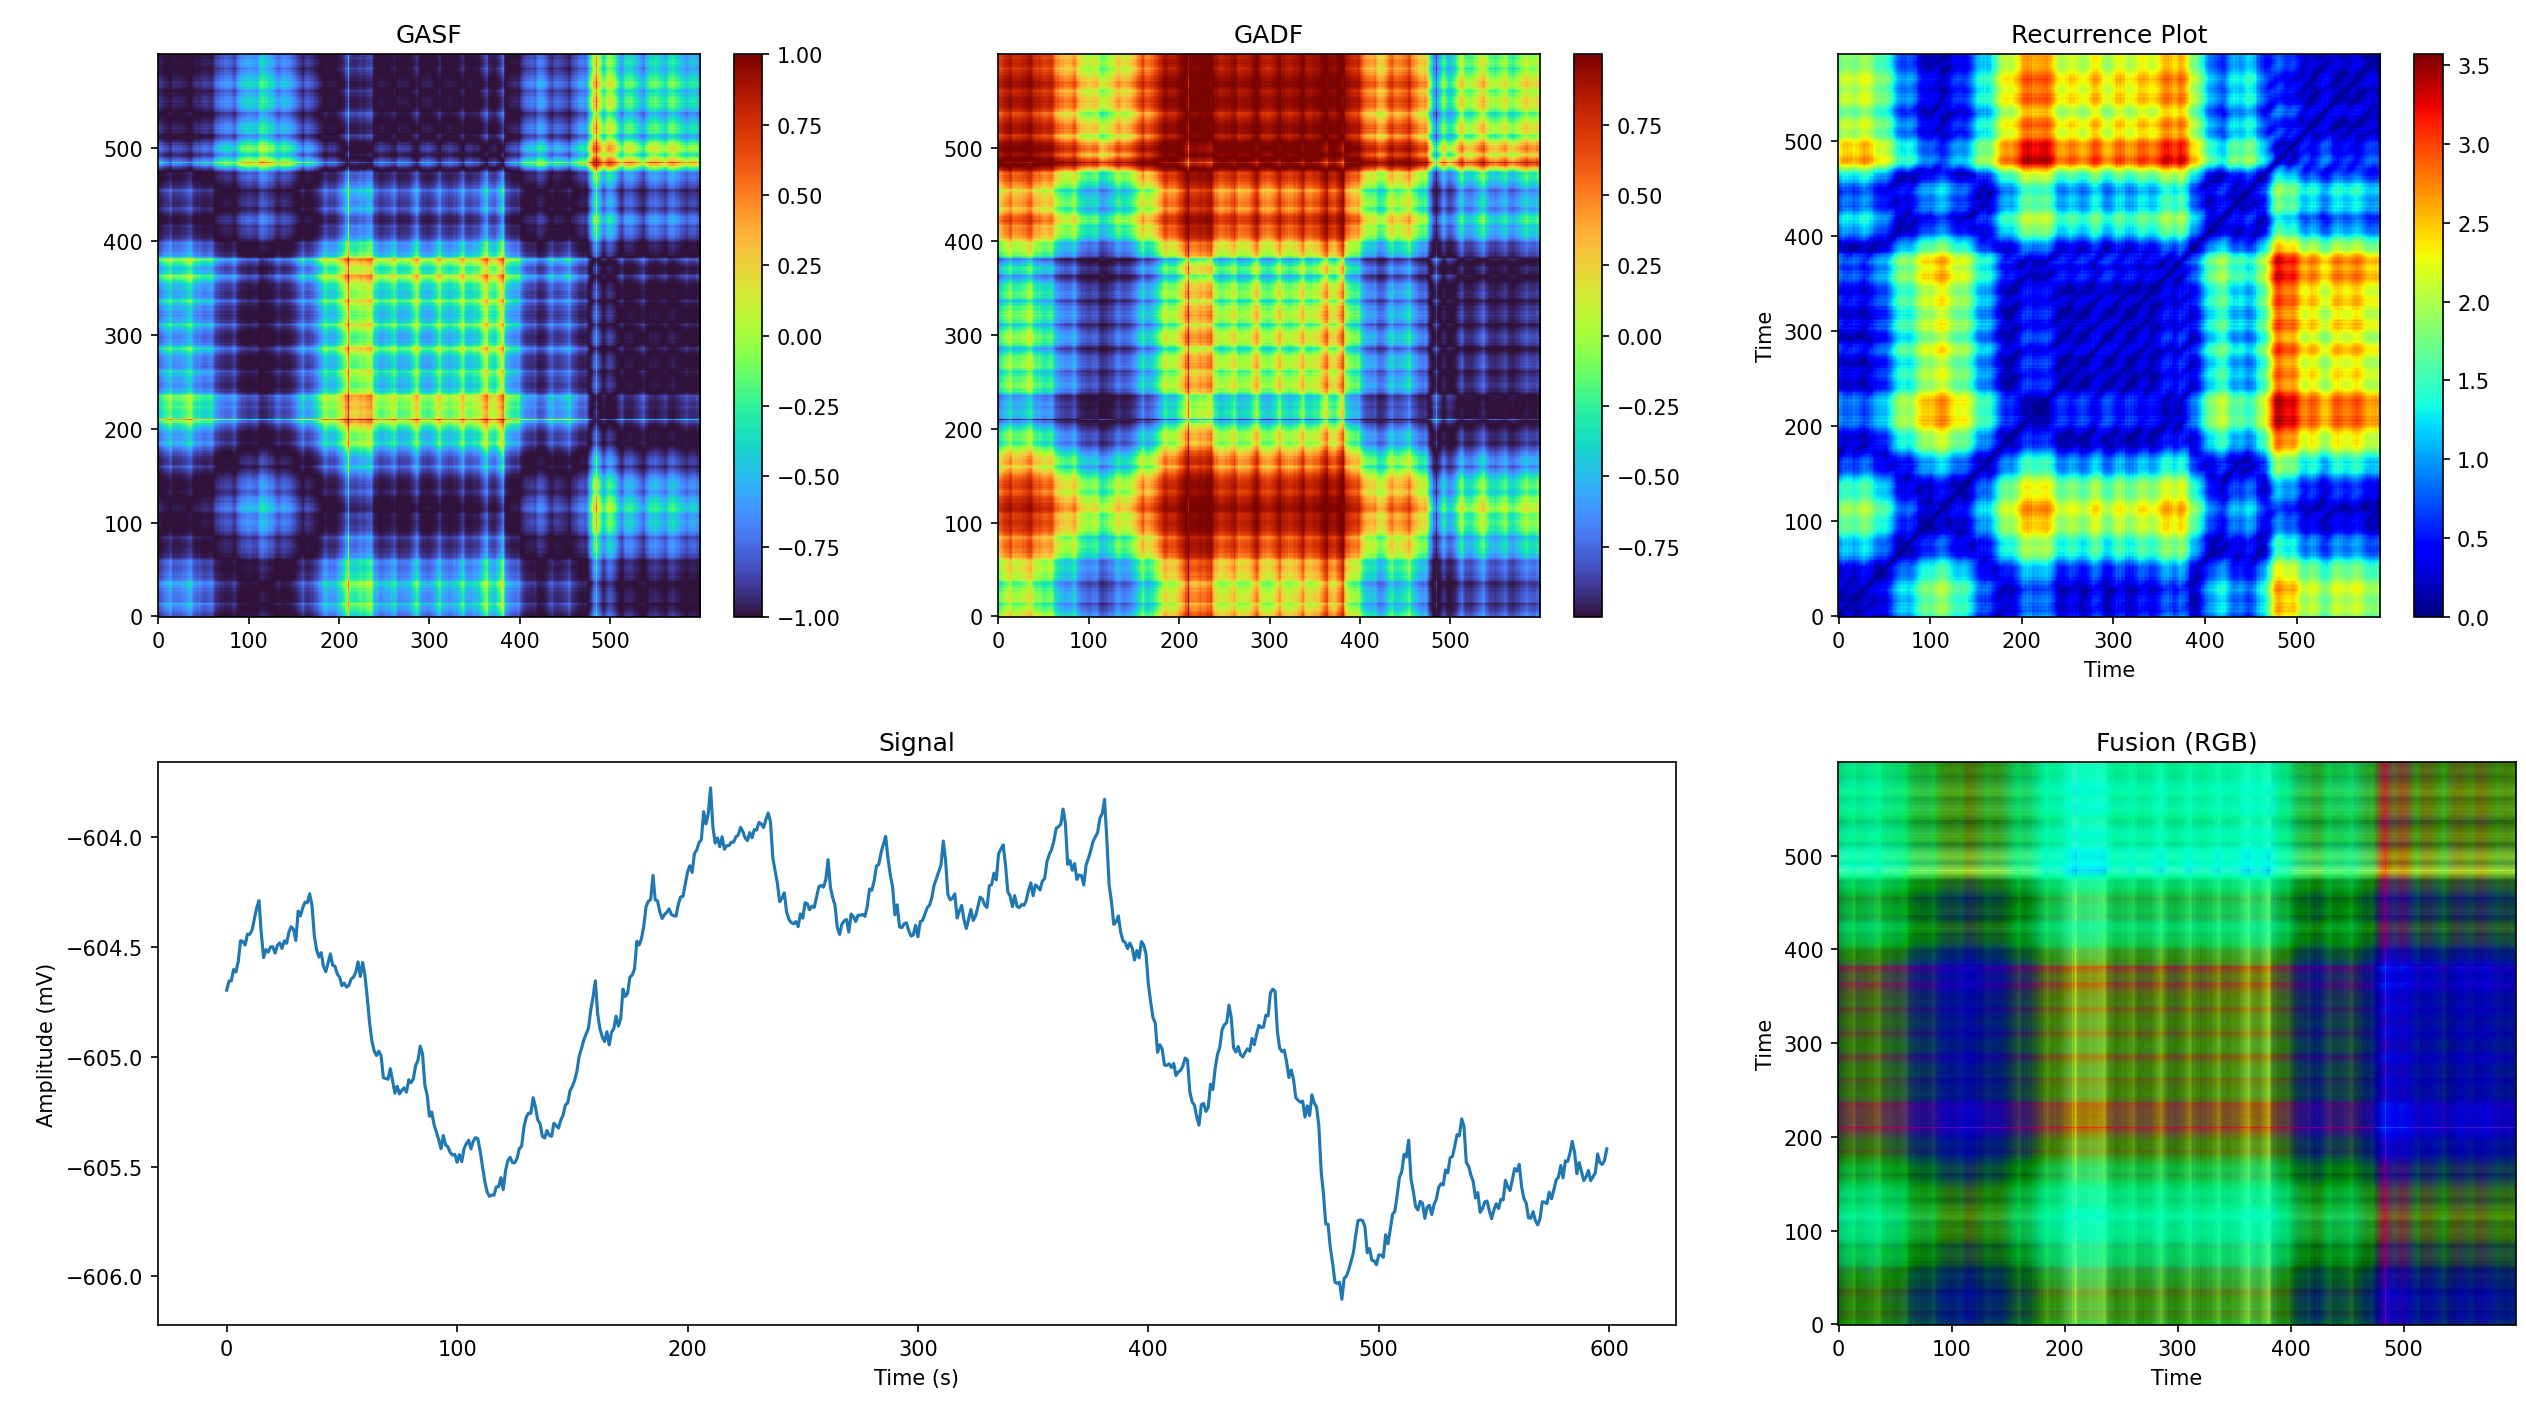
\includegraphics[width=\textwidth]{encodings/cnn_eg.png}
\caption{One 600-second window encoded as a GASF, a GADF, a recurrence plot and their RGB fusion, the four inputs of the CNN models.}
\label{fig:encodings}
\end{figure}

\begin{instructions}
Keep this figure here, with the theory; Chapter~\ref{ch:early} shows real labelled windows. Optionally redraw it in the
thesis figure style.
\end{instructions}

A further consideration for the CNN approach in this domain is the bootstrap problem: supervised classifiers require labelled training data, which does not currently exist in any standardised form for mycelium signals. Initial labels must therefore be generated by unsupervised methods before a classification model can be trained and evaluated. This is the role that matrix profiling and clustering are intended to play within the pipeline, which connects this section to Section~\ref{sec:litmp} and to the proposed methodology.

\section{Classification without hand-crafted features}
\label{sec:litclassifiers}
\label{sec:minirocket}

\begin{instructions}
New section, about half a page. Cover:
\begin{itemize}
  \item ROCKET \cite{dempster2020rocket} and MiniRocket \cite{dempster2021minirocket}: thousands of fixed random
        convolution kernels, with only a linear classifier trained on top, near state of the art on the UCR benchmarks
        at a fraction of the cost.
  \item catch22 \cite{lubba2019catch22}, a canonical set of 22 time-series features, used with random forests
        \cite{breiman2001rf}.
  \item EfficientNet \cite{tan2019efficientnet}, the CNN backbone of the image-encoded models.
\end{itemize}
Why these three: they span hand-designed features, random features and learned features, so a comparison between them
asks what kind of structure the labels carry.
\end{instructions}

\begin{instructions}
New section, about half a page. MiniRocket \cite{dempster2021minirocket} transforms a series with a fixed set of 84
convolution kernels of length 9 (weights from $\{-1, 2\}$), each applied at a range of dilations so that one kernel can
see 9 consecutive samples or a pattern spread over a minute or more. Each kernel--dilation pair is given biases taken
from the data's own quantiles, and contributes one feature: the proportion of positive values (PPV) of its convolution
output.
\begin{itemize}
  \item About 10,000 features result; none is learned.
  \item A ridge classifier is fitted on top. Here it is class-balanced, and Platt scaling \cite{platt1999} maps its
        score to a probability.
  \item In R4 the series is the detected span plus 25\,\% context each side, reduced to 512 points by bin means and
        z-normalised. Four scale features (log duration, peak-to-peak, noise, and their ratio) are appended.
\end{itemize}
Check the exact feature count in \src{DATA/derived/models/rq1b_minirocket/20261020-2343/manifest.json}.
\end{instructions}

\section{Detectors borrowed from other fields}
\label{sec:litdetectors}

\begin{instructions}
About one page. Updated 5 Nov. For each detector family in the sweep (Chapter~\ref{ch:rq1}), one short paragraph:
what it was built for and in which field, what it assumes about the signal, and why it might suit fungal recordings.
\textbf{Cite the source paper of each.} Chapter~\ref{ch:pipeline} then shows six of them on one sample signal
(Figure~\ref{fig:sixdetectors}) and as templates on the site.
\begin{itemize}
  \item OASIS deconvolution, from calcium imaging \cite{friedrich2017oasis}: a spike train convolved with an
        exponential decay, i.e.\ a jump followed by recovery.
  \item BEADS, from chromatography \cite{ning2014beads}: sparse peaks on a drifting baseline.
  \item The Dehshibi--Adamatzky wavelet detector \cite{dehshibi}, ported from the authors' own code
        \cite{dehshibi2020code}: the in-field contrast.
  \item Continuous-wavelet ridge peak detection, from mass spectrometry \cite{du2006cwt} (\texttt{cwt\_events}, B9).
  \item The matrix-profile threshold \cite{yeh} and symbol search over SAX strings \cite{lin2007sax}.
  \item Change-point detection \cite{truong2020ruptures} and FLUSS segmentation \cite{gharghabi2017fluss}.
  \item Interval measures for trains: burst detection by logISI \cite{pasquale2010logisi}, and the irregularity
        measures CV2 \cite{holt1996cv2} and LV \cite{shinomoto2003lv}, from neuroscience (B1).
  \item Wavelet scattering \cite{bruna2013scattering}.
\end{itemize}
One line each for the in-house detectors, which have no outside source: the drop detector (v1 and v5), deconvolved
troughs, the noise and signal thresholds, the wavelet-encoded detector and the CNN window scores. Multiscale entropy is
no longer reported (B7 was not run), so leave it out. Sources for the block designs:
\src{docs/research/analysis-blocks-from-literature.md} and \src{docs/research/analysis-blocks-primary-sources.md}.
\end{instructions}


\section{Distance, normalisation and scale invariance}
\label{sec:distance}

Every method in this thesis that groups, matches or retrieves a subsequence does so by way of a distance function, and the choice of that function determines what the method is capable of considering ``the same shape''. This section states the distances used and what each is invariant to, because RQ3 is precisely a question about invariance.

For two subsequences $Q = q_1,\ldots,q_m$ and $C = c_1,\ldots,c_m$ of equal length $m$, the Euclidean distance is
\begin{equation}
d(Q,C) = \sqrt{\sum_{i=1}^{m}(q_i - c_i)^2}.
\end{equation}
This is sensitive to both the offset and the amplitude of the two subsequences: a shape occurring during a slow depolarisation drift will be distant from an identical shape occurring at a different baseline, purely because of the offset. Since mycelium recordings exhibit exactly this kind of slow baseline wander, raw Euclidean distance is unsuitable for shape comparison.

The standard remedy is to z-normalise each subsequence before comparison. Writing $\hat{q}_i = (q_i - \mu_Q)/\sigma_Q$ for the mean $\mu_Q$ and standard deviation $\sigma_Q$ of $Q$, the z-normalised Euclidean distance is
\begin{equation}
d_z(Q,C) = \sqrt{\sum_{i=1}^{m}(\hat{q}_i - \hat{c}_i)^2},
\label{eq:znorm}
\end{equation}
which is invariant to offset and to amplitude scaling, and which is the distance the matrix profile is defined over \cite{yeh}. Equation \eqref{eq:znorm} is therefore the default distance throughout this thesis, and where a result is reported against an unnormalised comparison this is stated explicitly.

What Equation \eqref{eq:znorm} is \emph{not} invariant to is duration. Both subsequences must have the same length $m$, and a shape that occurs over four minutes in one region and over twelve minutes in another is not recoverable by a query defined at either length. This matters here more than it does in most domains: multiple scales of oscillatory behaviour are a documented characteristic of these signals \cite{adamatzky2023}, \cite{dehshibi}, and the same morphology has been observed by eye at durations differing by an order of magnitude. Three families of approach address this:

\begin{itemize}
  \item \textbf{Elastic distances}, of which Dynamic Time Warping is the canonical example, allow a non-linear alignment between the time axes of $Q$ and $C$, and so tolerate local stretching and compression. They are more expensive than Equation \eqref{eq:znorm} and admit alignments that are not always physically meaningful.
  \item \textbf{Resampling and uniform scaling}, in which the query is resampled to a range of candidate lengths and the best match across that range is retained. This is conceptually the simplest and is directly compatible with the matrix profile machinery, at the cost of a linear increase in computation with the number of scales searched.
  \item \textbf{Symbolic encodings} such as Symbolic Aggregate Approximation (SAX) \cite{lin2007sax}, which reduce a window to a short string of symbols via piecewise aggregate approximation followed by breakpoint quantisation of the z-normalised amplitude. Because the number of segments is fixed rather than the number of samples, the representation is intrinsically length-agnostic, and comparison becomes a string distance rather than a numerical one. A directional variant (dSAX) encodes the sign of change per segment (up, same, down). A pattern such as \texttt{U+ S? D+} then finds sharkfin-shaped events at any duration.
\end{itemize}

The architectural position taken in this thesis is that \emph{scale is a property of a motif, not of the analysis that discovered it}: every span carries its native duration, and every encoding declares whether or not it is scale-normalised. Whether a motif recurs at other scales is then a query that can be asked of the library, rather than an assumption baked into how the library was built.

\begin{instructions}
Settle the plan's open note on which scale-invariant distance is used. What the project ended with:
\begin{itemize}
  \item seeded search uses $d_z$ at the seed's own length;
  \item the Library offers four distances, including MPdist \cite{gharghabi2018mpdist} and a scale-invariant
        (resampled) distance;
  \item the RQ3 pilot banks searches at 0.8$\times$, 1$\times$ and 1.25$\times$;
  \item the drop-motif study resamples each event to a 200-point frame in units of its own fall.
\end{itemize}
Then state the key finding, which belongs here as theory and in Chapter~\ref{ch:events} as evidence: resampling to a
fixed length removes absolute duration and amplitude but not measurement resolution. The normalised vector still
predicts how many samples an event was built from, at 0.753 balanced accuracy against a chance of 0.25
(\src{Plots/drop_motifs10/CLAIMS.md}, row 9). Normalisation is therefore not the same as invariance.
\end{instructions}

\section{Surrogate data and null hypothesis testing}
\label{sec:litsurrogates}
\label{sec:surrogates}

\begin{instructions}
New section, about half a page. The method of surrogate data \cite{theiler1992surrogate}; amplitude-adjusted and
iterated surrogates \cite{schreiber1996iaaft,schreiber2000surrogate}; their use in EEG and physiology to separate linear
spectral structure from anything more. Make the point for the fungal field: none of the reviewed fungal studies reports
a detector's output against a surrogate of the same signal.
\end{instructions}

A motif discovery algorithm applied to any sufficiently long signal will return motifs. The matrix profile in particular is guaranteed to return the most similar pair of subsequences in a dataset, whether or not that pair is meaningfully similar --- the guarantee is on optimality of the search, not on significance of the result. Reporting that recurring structure was found is therefore not by itself evidence that the signal contains structure. What is required is a null: how much structure of this kind does the same method recover from a signal that is known to contain none of the structure of interest, but is otherwise comparable?

Surrogate data testing supplies that null \cite{theiler1992surrogate}. A surrogate is a synthetic series generated from the original recording so as to preserve certain statistical properties while destroying others. Comparing a statistic computed on the original against the distribution of the same statistic computed on an ensemble of surrogates gives a test of the specific hypothesis that the surrogate generation was designed to destroy.

Three surrogate types are used in this thesis.

\textbf{Phase-randomised surrogates} preserve the power spectrum, and therefore the linear autocorrelation structure, while destroying the phase relationships that give rise to specific waveform shapes. Given a recording $x$ of length $n$, the discrete Fourier transform $X_k$ is computed, the phase of each coefficient is replaced by a value drawn uniformly from $[0, 2\pi)$ subject to conjugate symmetry, and the inverse transform is taken:
\begin{equation}
\tilde{x} = \mathcal{F}^{-1}\!\left\{ |X_k| \, e^{i\phi_k} \right\}, \qquad \phi_k \sim U[0,2\pi).
\end{equation}
The result has the same spectrum and the same autocorrelation as the original, and is a linear Gaussian process in every other respect. A motif recovered from the original but not from its phase-randomised surrogate is therefore evidence of structure that is not explained by the signal's spectral content alone --- which is the relevant null for this project, since slow drifts and broad oscillatory content are known to be present and are not what is being claimed.

\textbf{Amplitude-adjusted (AAFT) surrogates} \cite{theiler1992surrogate,schreiber2000surrogate} also preserve the recording's distribution of values, by rank-remapping a phase-randomised Gaussian series onto the original amplitudes. They are the right null for value-reading measures such as multiscale entropy, where a phase-randomised surrogate would differ from the original in its amplitude distribution as well as its structure.

\textbf{Block-shuffled surrogates} preserve short-range structure within blocks while destroying the ordering between them. The recording is partitioned into contiguous blocks and the blocks are randomly permuted. This provides a complementary null for questions concerning the arrangement of events in time --- such as whether events recur at intervals that are themselves structured --- where phase randomisation would be too destructive to be informative.

In every case, the surrogate is not a different experiment. The identical analytical chain is rerun on the surrogate at identical parameters, and the comparison reported is between two runs of the same recipe. This is implemented in \tool{} as a \texttt{Signal $\rightarrow$ Signal} block (Section~\ref{sec:types}), precisely so that the comparison is cheap enough to run routinely. Figure~\ref{fig:nullviolin} shows a worked example.

\begin{figure}[htbp]
\centering
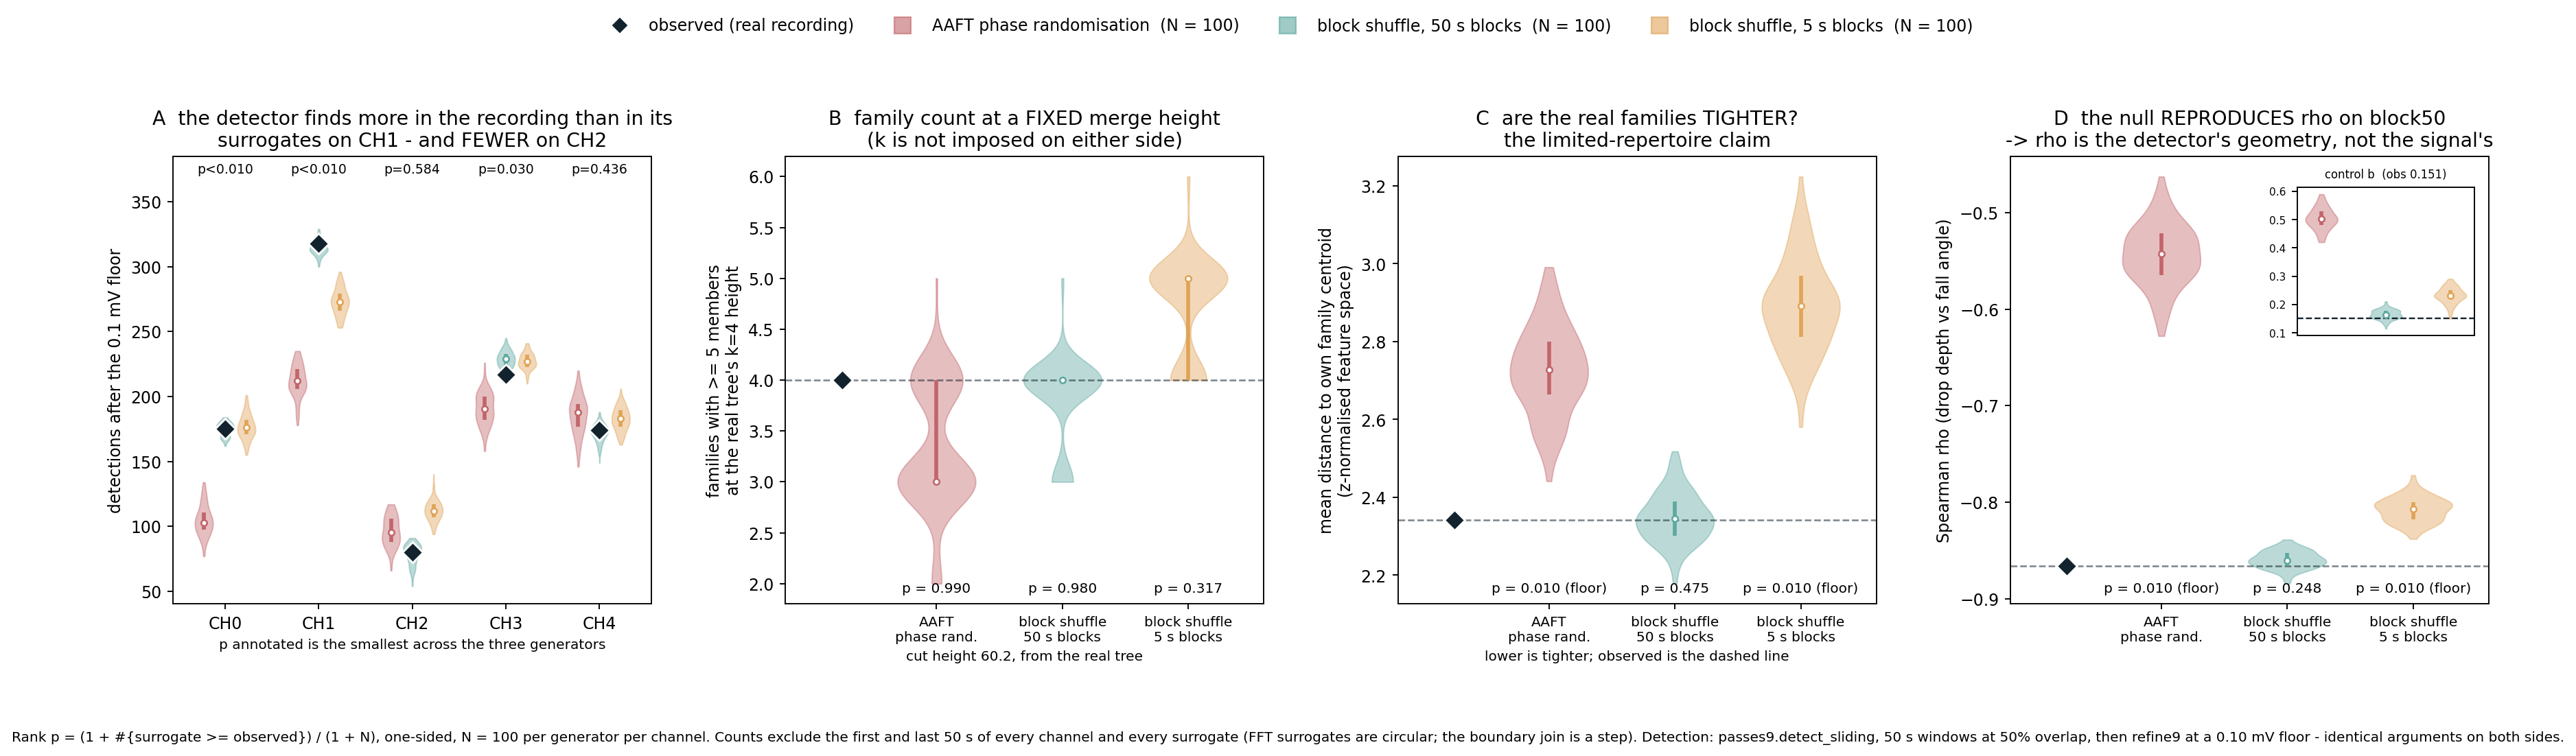
\includegraphics[width=\textwidth]{drop_motifs/NULL_surrogate.png}
\caption{A worked surrogate test from the drop-motif study: observed statistics (detection count, family count, tightness, rank correlation) against AAFT and block-shuffled surrogates.}
\label{fig:nullviolin}
\end{figure}

\begin{instructions}
Settle the plan's two open decisions here.

Realisation counts, as actually used:
\begin{itemize}
  \item 1 draw per task in the detector sweep (cost; 20-draw re-runs on rangpur were prepared);
  \item 20 draws for the demonstration detector;
  \item 200 phase-randomised draws per channel for seed searches;
  \item 3--5 for Library quiet-window nulls;
  \item 200 label shuffles for every classifier null.
\end{itemize}
State the $p$-value floor, $1/(N+1)$: 0.005 at 200 draws. Coverage: 2,587 of 2,936 real runs carry at least one
surrogate, so ``every result'' is true of the reported results, not of every run ever made.

Reporting: rank-based $p$-values plus an effect size, either the real/surrogate ratio or a $z$ against the null
distribution.

Also say what a surrogate is never allowed to be: a detection counted as a finding
(\src{tests/test_surrogate_never_a_detection.py}).
\end{instructions}

\begin{figure}[htbp]
\centering
\figplaceholder{5cm}{Figure 2.3 (T1, bundle): six hours of one M2\_aug channel above its AAFT copy and a
block-shuffled copy, on the same axes. The copies keep the values (and, for AAFT, the spectrum) but not the shapes.}
\caption{What a null looks like: a recording beside two of its surrogates.}
\label{fig:surrogateexample}
\end{figure}

\section{Human judgement as ground truth}
\label{sec:lithuman}

\begin{instructions}
New section, about half a page.
\begin{itemize}
  \item Where no labels exist, a human's verdict is the reference, so its reliability has to be measured: intra-rater
        agreement and Cohen's $\kappa$ \cite{cohen1960kappa}.
  \item Blind presentation, and stratified sampling so rare strata are seen.
  \item Proportions with Wilson intervals \cite{wilson1927}; differences with Newcombe's method \cite{newcombe1998}.
  \item This project's own number: you agree with yourself on 94\,\% of 98 blind repeats ($\kappa$ 0.84). That is the
        ceiling any classifier can be measured against.
\end{itemize}
\end{instructions}

\section{Evaluation statistics}
\label{sec:stats}

\begin{instructions}
New section, about one page. Define each statistic once, with the formula and a one-line ``what it answers'':
\begin{itemize}
  \item Precision $=\mathrm{TP}/(\mathrm{TP}+\mathrm{FP})$, the share of a detector's candidates you judged real, with a
        Wilson 95\,\% interval \cite{wilson1927}.
  \item Stratified estimation: the share real across a table of candidate events, estimated from a stratified sample
        weighted by stratum size, with a bootstrap interval \cite{efron1979bootstrap} (1,000--2,000 resamples).
  \item AUC, the probability that a real event outscores a non-event. It does not depend on a cut.
  \item Balanced accuracy, the mean of sensitivity and specificity, robust to the 80:20 imbalance of the 10-minute labels.
  \item Macro F1.
  \item Cohen's $\kappa$ \cite{cohen1960kappa}, for your re-test agreement.
  \item Label-shuffle permutation nulls (labels permuted within recording and kind, the whole fit repeated).
  \item Leave-one-recording-out cross-validation.
  \item Cramér's V \cite{cramer1946}, for family-by-label association.
  \item The cophenetic correlation \cite{sokal1962cophenetic}, for how faithfully a Ward tree \cite{ward1963}
        summarises its distances.
  \item Newcombe's interval for a difference of proportions \cite{newcombe1998} and Fisher's exact test (blind panel).
\end{itemize}
Note why accuracy is not reported alone: a model that always answers ``not interesting'' scores about 0.79--0.81
accuracy on the 10-minute labels.
\end{instructions}

\section{Gaps in knowledge}
\label{sec:litgaps}

The literature reviewed in this chapter reveals three interconnected gaps that the present project is designed to address.

The first is the absence of modern time-series analysis methods in the study of fungal bio-electric signals. Despite the rapid growth of these methods in related domains --- including EEG analysis, power systems monitoring, and respiratory biology --- no published work has applied matrix profiling or image-based CNN classification to mycelium recordings. The analyses that do exist are bespoke, manually parameterised, and not released in reproducible form \cite{dehshibi}, \cite{buffi}, meaning the body of findings cannot be built upon incrementally.

The second, and arguably more fundamental, gap is the lack of a foundational classification framework for mycelium signal types. Individual studies describe oscillatory behaviour at multiple time-scales \cite{adamatzky2023}, \cite{dehshibi}, identify spike-trains with varying morphology \cite{slayman}, \cite{adamatzky2022}, and note species-specific differences in signal complexity \cite{adamatzky2022}, but no study has attempted to define a reproducible taxonomy of signal states. Without such a taxonomy, supervised learning approaches cannot be validated across datasets, and findings from one species or experimental condition cannot be compared with those from another. This mirrors a challenge that the EEG field resolved through the establishment of canonical sleep-staging definitions, which subsequently enabled decades of automated classifier development. For mycelium signals, that equivalent groundwork has not been laid.

The third gap is the absence of a shared computational pipeline that a researcher can use to interrogate a new recording. Existing tools are described only in methods sections, are not released, and are not designed to be repurposed. A researcher studying a new species or a new experimental condition currently has no standard starting point for analysis. The present project is designed to address all three of these gaps in a single integrated framework.

\begin{instructions}
Add the fourth gap if you used it in Section~\ref{sec:gaps}: no fungal study measures any detector's precision against
blind human judgement, or against a surrogate of the same signal. That is the gap RQ1 fills.
\end{instructions}
